\documentclass[10pt]{article}

%------------------------------------------------------
%   PACKAGES
%------------------------------------------------------

% Default 
\usepackage{graphicx}
\usepackage[backend=biber,style=numeric,sorting=none]{biblatex}

% Additional
\usepackage{amsmath}
\usepackage{textcomp, gensymb}
\usepackage{placeins}
\usepackage{tabularray} 
\usepackage{xcolor}
\usepackage{placeins}
\usepackage{todonotes}
\usepackage{parskip}
\newcommand{\td}[1]{\todo[linecolor=blue, backgroundcolor=blue!25,bordercolor=blue, size=\small]{#1}}

\addbibresource{references.bib}

\title{Microwave Optics I} 
\author{Rahmanyaz Annyyev, Hikmat Gulaliyev} 
\date{17 March 2024} 

\begin{document}

\maketitle

\begin{abstract}

\end{abstract}

\section{Introduction}

The electromagnetic spectrum is the range of all possible frequencies of electromagnetic radiation. The spectrum is divided into several regions, in order of decreasing frequency and increasing wavelength: gamma rays, X-rays, ultraviolet, visible light, infrared, microwaves, and radio waves. The microwave region of the electromagnetic spectrum is usually defined as being the range of frequencies from 1 GHz to 100 GHz. The wavelengths of microwaves are usually measured in centimeters. Microwaves are widely used in modern technology, for example in telecommunications, radar, and microwave ovens. The primary goal of this experiment is to verify the wave nature of microwaves.

The experiment is divided into three parts: A, B, and C. The experimental setup is comprised of a microwave transmitter with a Gunn diode, a microwave receiver with a Schottky diode, a goniometer, three dielectric perspex blocks, a metal reflector, and a polarization grille.

Standing waves are a type of wave that occurs when two waves of the same frequency and amplitude travel in opposite directions and interfere with each other. They are characterized by nodes and antinodes. A node is a point on a standing wave where the wave has zero amplitude. An antinode is a point on a standing wave where the amplitude is at a maximum. The distance between two consecutive nodes or antinodes is equal to half the wavelength of the wave and is denoted by $\lambda/2$.

In part A of the experiment, we employ this property of standing waves to measure the wavelength of microwaves. The experimental setup is shown in Figure~\ref{fig:1}.
We use a microwave transmitter and receiver to detect the standing waves and then measure the distance between two consecutive antinodes to determine the wavelength of the microwaves.

\begin{figure}[ht]
  \centering
  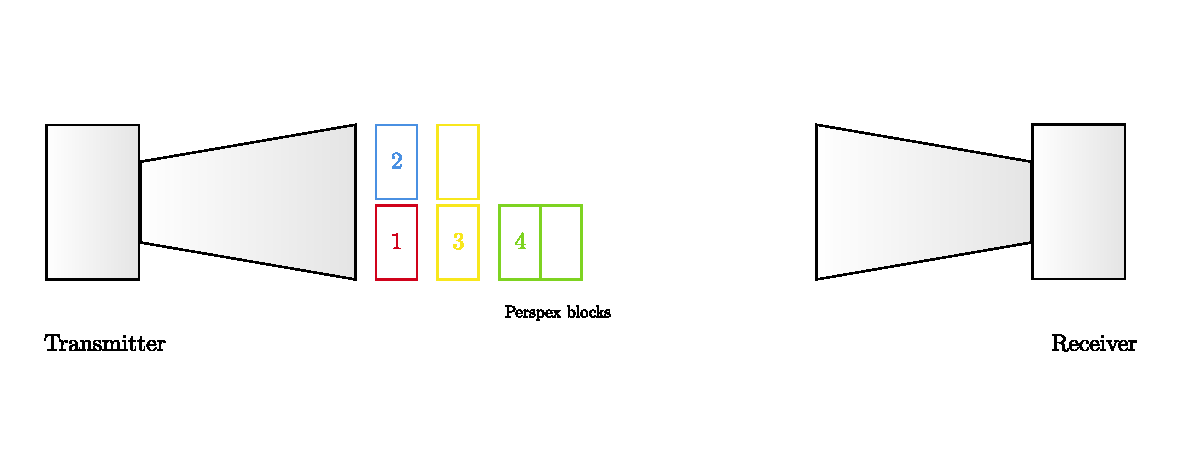
\includegraphics[scale=0.4]{figures/f1.pdf}
  \caption{Experimental setup for part A.}
  \label{fig:1}
\end{figure}

The speed of electromagnetic wave propagation in vacuum is denoted by $c$ and is approximately $3 \times 10^8$ m/s. As the wave enters a dielectric material, the speed of propagation decreases. This is due to the interaction of the electromagnetic wave with the atoms and molecules of the material; the electric and magnetic fields of the wave cause the charges in the material to move, which in turn generates new electromagnetic waves. The superposition of the original wave and the new waves results in a decrease in the speed of propagation. The speed of propagation in a dielectric material is denoted by $v$ and is given by the equation
\begin{equation}
  v = \frac{c}{n},
\end{equation}
where $n$ is the refractive index of the material. In part B of the experiment, we use a dielectric material to reduce the speed of propagation of microwaves and measure it. The setup is shown in Figure~\ref{fig:2}.

\begin{figure}[ht]
  \centering
  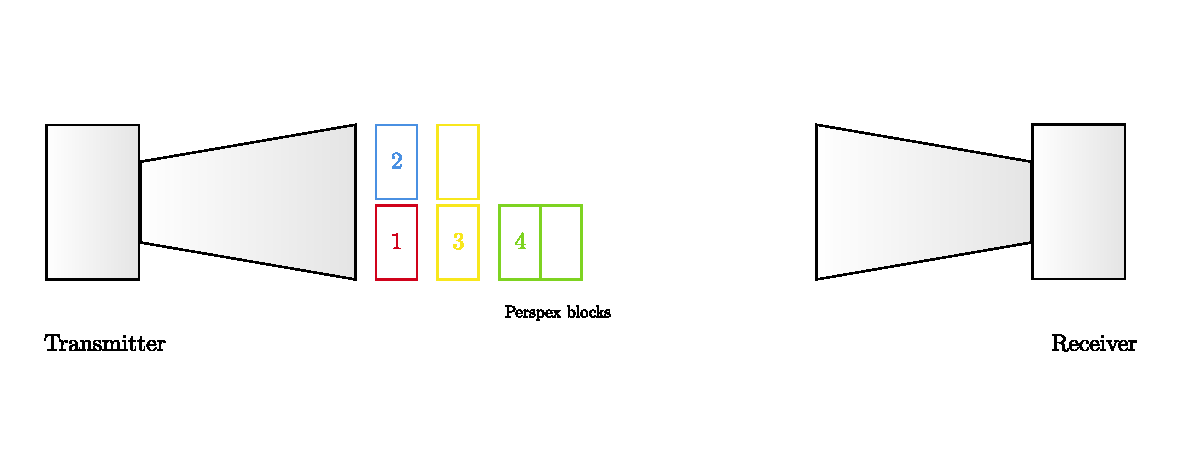
\includegraphics[scale=0.4]{figures/f2.pdf}
  \caption{Experimental setup for part B.}
  \label{fig:2}
\end{figure}

The polarization of an electromagnetic wave is the orientation of the electric field vector. The polarization of a wave can be linear, circular, or elliptical. In part C of the experiment, we use a polarization grille to change the polarization of microwaves and measure the effect of the grille on the intensity of the microwaves. The setup is shown in Figure~\ref{fig:3}.

\begin{figure}[ht]
  \centering
  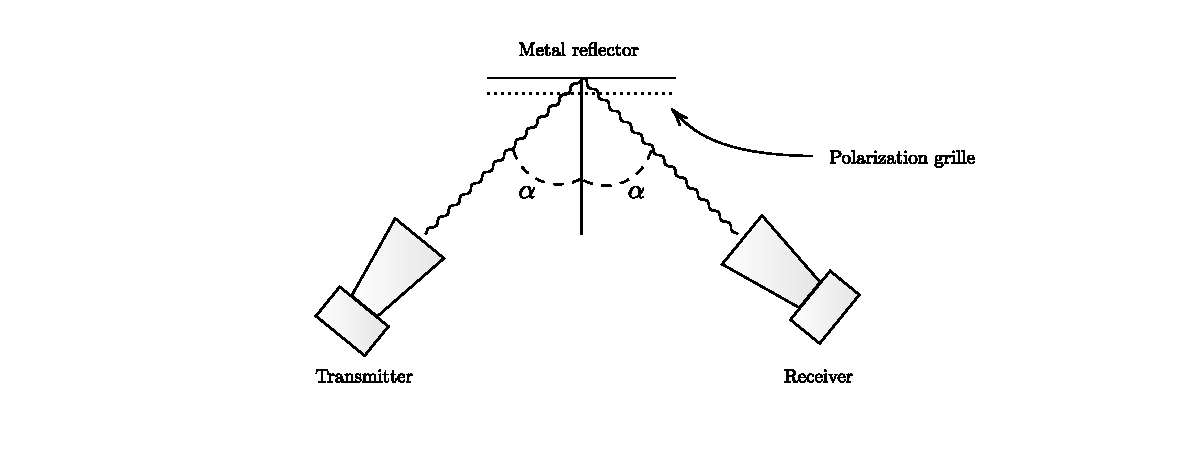
\includegraphics[scale=0.6]{figures/f3.pdf}
  \caption{Experimental setup for part B.}
  \label{fig:3}
\end{figure}

\section{Data \& Results}

The results of part A are shown in Table~\ref{tab:1}. The average value of the wavelength of microwaves is found to be $\bar{\lambda} = 2.925$ cm. 

\begin{table}[ht]
  \label{tab:1}
  \centering
  \vspace{4mm}

  \begin{tblr}{
    cells = {halign = c, valign = m},
    row{odd} = {bg = lightgray!5},
    row{1} = {bg = lightgray!20},
    hlines = {},
    vlines = {}
  }
    $i$ & 1 & 2 & 3 & 4 & 5 & 6 & 7 & 8 & 9 \\
    $x_i$ (cm) & 94 & 92.5 & 91.5 & 89.5 & 88 & 86.7 & 85.3 & 83.7 & 82.3 
  \end{tblr}
  \caption{Data for standing waves, part A.}
\end{table}

The results of part C are shown in Table~\ref{tab:2}.

\begin{table}[ht]
  \label{tab:2}
  \centering
  \vspace{4mm}

  \begin{tblr}{
    cells = {halign = c, valign = m},
    row{odd} = {bg = lightgray!5},
    row{1} = {bg = lightgray!20},
    hlines = {},
    vlines = {}
  }
    Receiver angle, $\theta$ & 0\degree & 45\degree & 90\degree & 135\degree & 180\degree & 225\degree & 270\degree & 315\degree \\
    Intensity, $I$ & 0.5 & 0.4 & 0.3 & 0.2 & 0.1 & 0.2 & 0.3 & 0.4 \\
    Setting & $10\times$ & $30\times$ & $30\times$ & All & $10\times$ & $3\times$ & $30\times$ & All
  \end{tblr}
  \caption{Data for polarization, part C.}
\end{table}


\section{Discussion \& Conclusion}

% \printbibliography

\end{document}